\documentclass[handout]{beamer}
\usepackage{handoutWithNotes}
%
%  Load other packages you may need here
% 
% \pgfpagesuselayout{4 on 1}[a4paper,landscape,border shrink=5mm
\pgfpagesuselayout{4 on 1 with notes}[a4paper,border shrink=5mm]
\usetheme{CambridgeUS}
\usecolortheme{seagull}
\usefonttheme{professionalfonts}
\usepackage{amssymb,amsmath}
\usepackage{ifxetex,ifluatex}
\usepackage{fixltx2e} % provides \textsubscript
\usepackage{lmodern}
\ifxetex
  \usepackage{fontspec,xltxtra,xunicode}
  \defaultfontfeatures{Mapping=tex-text,Scale=MatchLowercase}
  \newcommand{\euro}{€}
\else
  \ifluatex
    \usepackage{fontspec}
    \defaultfontfeatures{Mapping=tex-text,Scale=MatchLowercase}
    \newcommand{\euro}{€}
  \else
    \usepackage[T1]{fontenc}
    \usepackage[utf8]{inputenc}
      \fi
\fi
\IfFileExists{upquote.sty}{\usepackage{upquote}}{}
% use microtype if available
\IfFileExists{microtype.sty}{\usepackage{microtype}}{}

% Comment these out if you don't want a slide with just the
% part/section/subsection/subsubsection title:
\AtBeginPart{
  \let\insertpartnumber\relax
  \let\partname\relax
  \frame{\partpage}
}
\AtBeginSection{
  \let\insertsectionnumber\relax
  \let\sectionname\relax
  \frame{\sectionpage}
}
\AtBeginSubsection{
  \let\insertsubsectionnumber\relax
  \let\subsectionname\relax
  \frame{\subsectionpage}
}

\setlength{\parindent}{0pt}
\setlength{\parskip}{6pt plus 2pt minus 1pt}
\setlength{\emergencystretch}{3em}  % prevent overfull lines
\setcounter{secnumdepth}{0}

\title{Constrained Parenting Decisions}
\author{Joe Mienko}
\date{Wednesday, October 23, 2014}

\begin{document}
\frame{\titlepage}

\begin{frame}{Introduction}

\begin{itemize}[<+->]
\itemsep1pt\parskip0pt\parsep0pt
\item
  The purpose of this manuscript is to formally specify and test a
  general theory of child maltreatment.
\end{itemize}

\begin{itemize}[<+->]
\itemsep1pt\parskip0pt\parsep0pt
\item
  Well-known association between poverty and child maltreatment.
\end{itemize}

\begin{itemize}[<+->]
\itemsep1pt\parskip0pt\parsep0pt
\item
  Lack of a basic framework explaining why we would expect a link
  between poverty and child maltreatment.
\end{itemize}

\begin{itemize}[<+->]
\itemsep1pt\parskip0pt\parsep0pt
\item
  This study and the empirical analysis presented here attempt to
  provide such a basis.
\end{itemize}

\end{frame}

\begin{frame}{Background - Human Evolution}

\begin{block}{Why do Humans Engage in Parenting Activities?}

\begin{itemize}[<+->]
\itemsep1pt\parskip0pt\parsep0pt
\item
  Basic evolutionary theory demonstrates that behaviors exist
  \emph{because} they helped genes to evolve to their present state.
\end{itemize}

\begin{itemize}[<+->]
\itemsep1pt\parskip0pt\parsep0pt
\item
  Parental altruism is one such behavior - defined as those behaviors
  requiring the investment of time or other resources in a child in a
  way that benefits the child but comes at a cost to the parent.
\end{itemize}

\begin{itemize}[<+->]
\itemsep1pt\parskip0pt\parsep0pt
\item
  By engaging in such altruistic acts to her own children, a parent is
  increasing the survival probability of her own children and thus
  increasing the survival probability of her own genes.
\end{itemize}

\end{block}

\end{frame}

\begin{frame}{Background - Human Evolution}

\begin{block}{Do Parents Engage in Altruism Forever?}

\begin{itemize}[<+->]
\itemsep1pt\parskip0pt\parsep0pt
\item
  No!
\end{itemize}

\begin{itemize}[<+->]
\itemsep1pt\parskip0pt\parsep0pt
\item
  Countless examples of infanticide in tribal cultures.
\end{itemize}

\begin{itemize}[<+->]
\itemsep1pt\parskip0pt\parsep0pt
\item
  Until recently, infanticide was regularly practiced in Western
  cultures.
\end{itemize}

\end{block}

\end{frame}

\begin{frame}{Parental Decision-Making}

\begin{block}{Why do Parents Make Different Decisions in Different
Circumstances?}

\begin{itemize}[<+->]
\itemsep1pt\parskip0pt\parsep0pt
\item
  Humans have agency (or at they at least act like they do)
\end{itemize}

\begin{itemize}[<+->]
\itemsep1pt\parskip0pt\parsep0pt
\item
  Evidence from neuroscience suggests that humans make decisions with
  both automaticity
\end{itemize}

\begin{itemize}[<+->]
\itemsep1pt\parskip0pt\parsep0pt
\item
  \ldots{}and as the result of more thoughtful deliberation.
\end{itemize}

\end{block}

\end{frame}

\begin{frame}{Parental Decision-Making}

\begin{block}{Joshua Greene's Dual Process Theory of Morality}

\begin{itemize}[<+->]
\itemsep1pt\parskip0pt\parsep0pt
\item
  Greene (2014) outlines a model of this dual-process human brain in
  which humans are said to possess an automatic mode (primarily driven
  by structures such as the ventromedial prefrontal cortex) and a manual
  mode (primarily driven by structures such as the dorsolateral
  prefrontal cortex).
\end{itemize}

\begin{itemize}[<+->]
\itemsep1pt\parskip0pt\parsep0pt
\item
  In simple terms, moral decisions that require cost-benefit analysis
  and thinking require humans to engage in manual mode, deliberative
  thinking.
\end{itemize}

\begin{itemize}[<+->]
\itemsep1pt\parskip0pt\parsep0pt
\item
  Moral decisions that do not require cost-benefit analysis are viewed
  to be made automatically - without the need for higher level thought
  processes.
\end{itemize}

\end{block}

\end{frame}

\begin{frame}{State Decision-Making}

\begin{block}{Why do State's Intervene in Family Lives?}

\begin{itemize}[<+->]
\itemsep1pt\parskip0pt\parsep0pt
\item
  Since the 19th century, Western society and most of the world has
  evolved into a series of social welfare states which also seek to
  prevent the existence of ``carnival{[}s{]} of slaughter''.
\end{itemize}

\begin{itemize}[<+->]
\itemsep1pt\parskip0pt\parsep0pt
\item
  When parent's violate this understanding, we tend to see children who
  are less well-developed and less capable of full participation in
  society as adults. In other words, society is made to pay for
  individual parental decisions.
\end{itemize}

\begin{itemize}[<+->]
\itemsep1pt\parskip0pt\parsep0pt
\item
  For the purposes of this manuscript, instances in which this contract
  is broken down are viewed to be instances of child maltreatment. When
  children are maltreated, the state is viewed to have a fiduciary
  obligation to both the child and to the rest of society.
\end{itemize}

\end{block}

\end{frame}

\begin{frame}{Overall Conceptual Model}

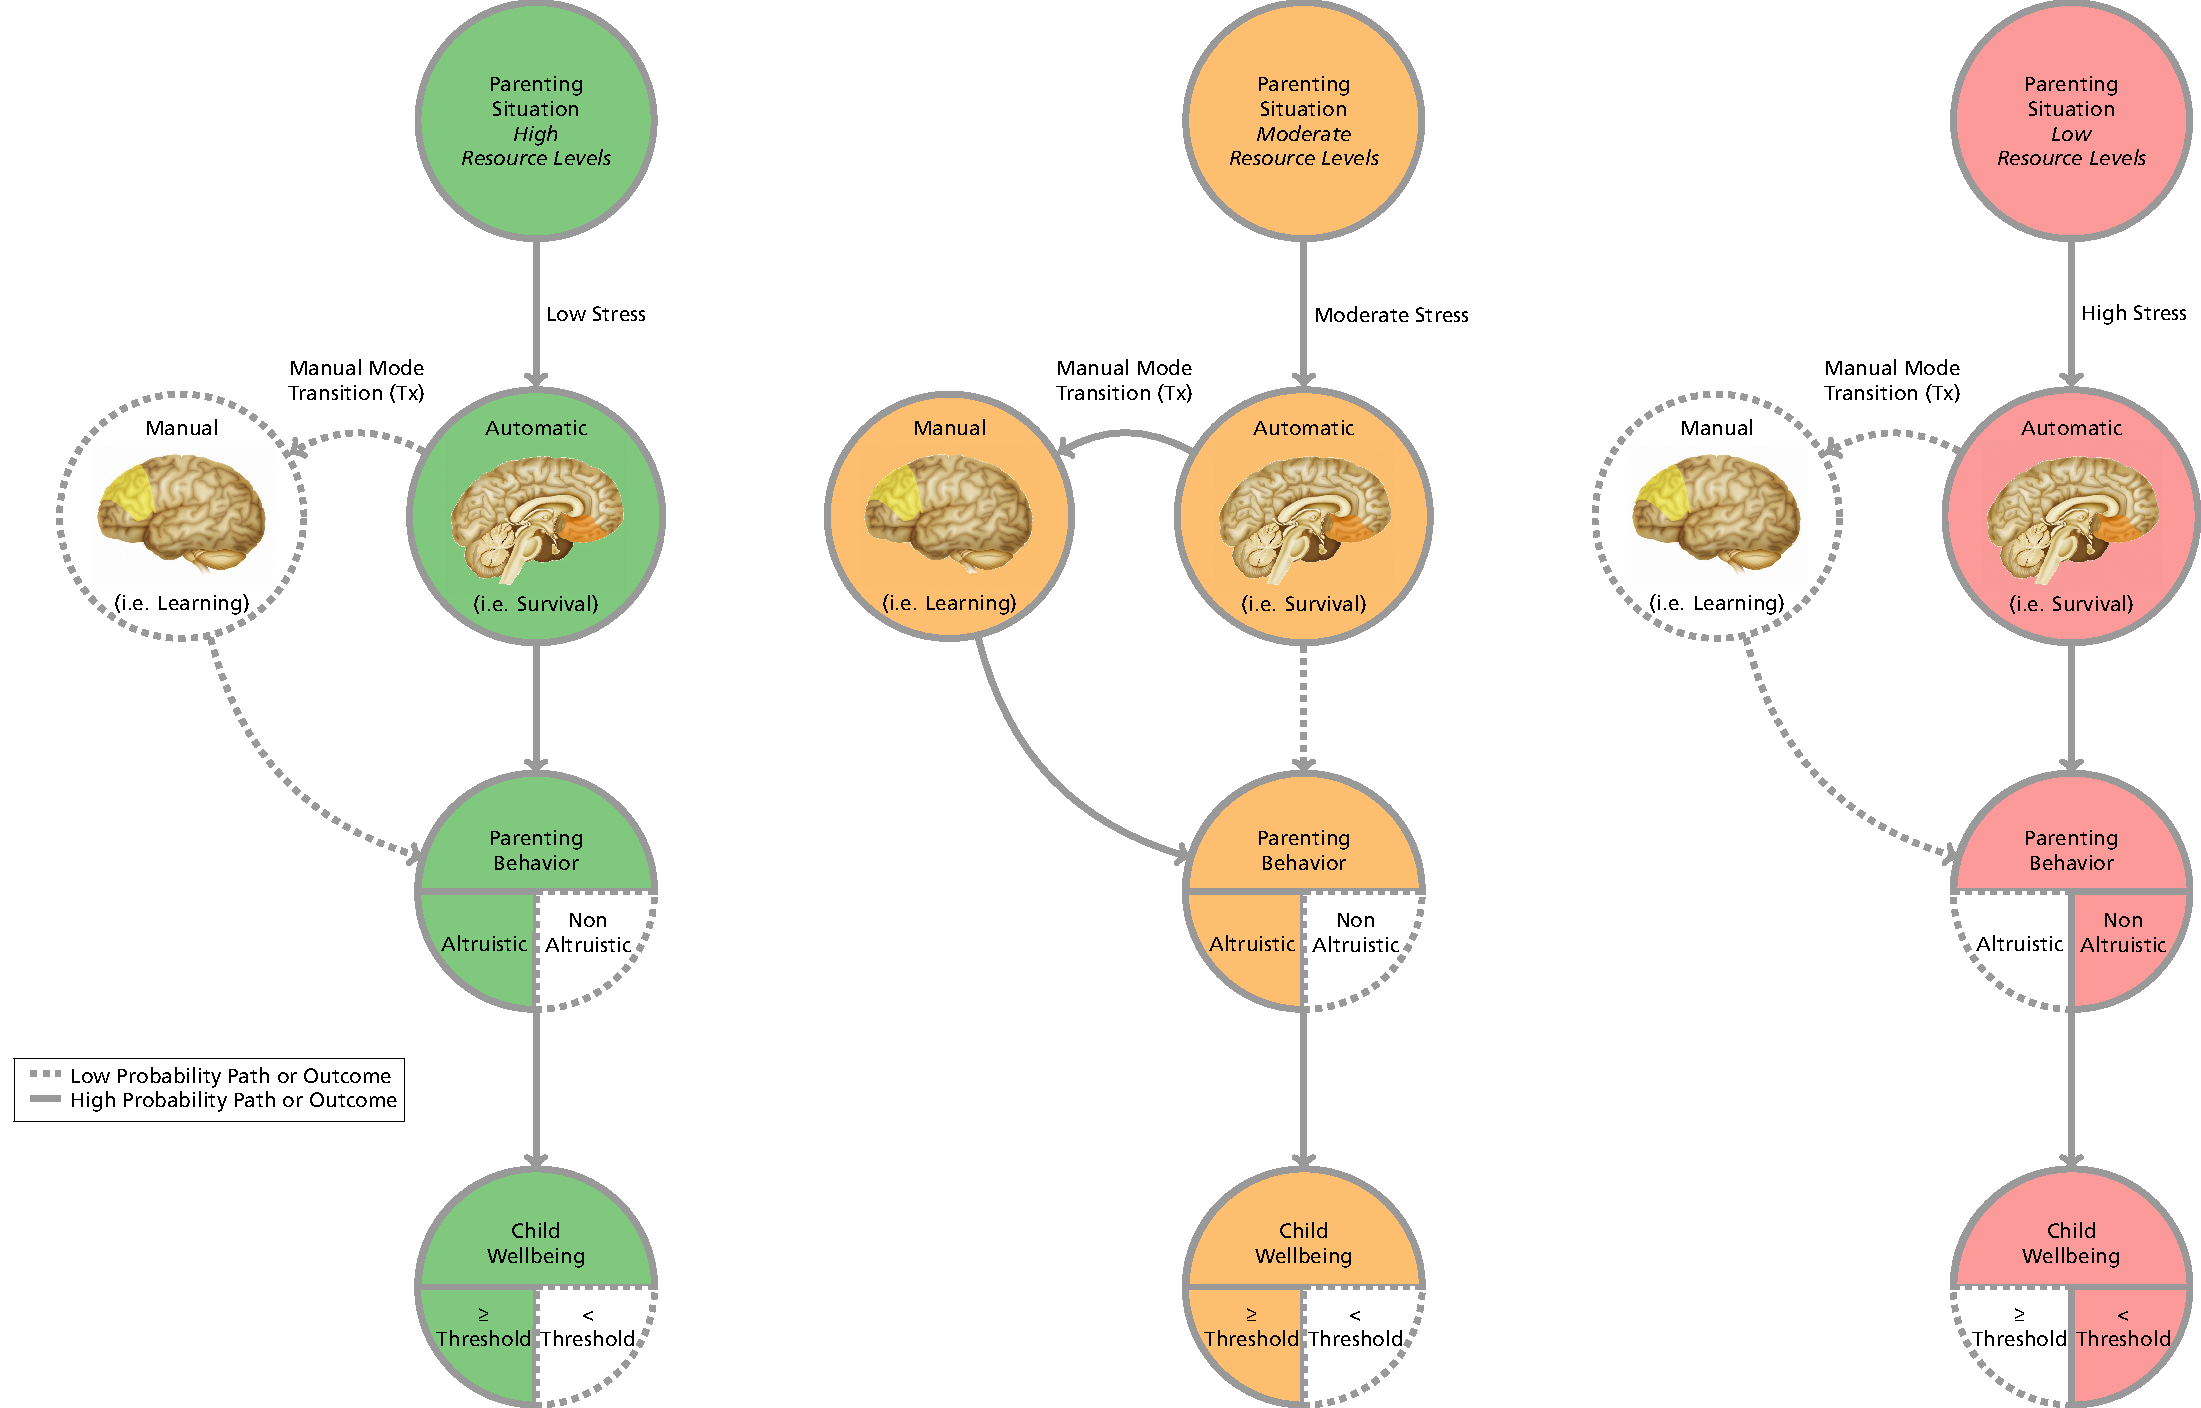
\includegraphics[scale=0.3]{general_conceptual_model_flow.pdf}

\end{frame}

\begin{frame}{Decisions Under Low Resource Levels}

\centering{
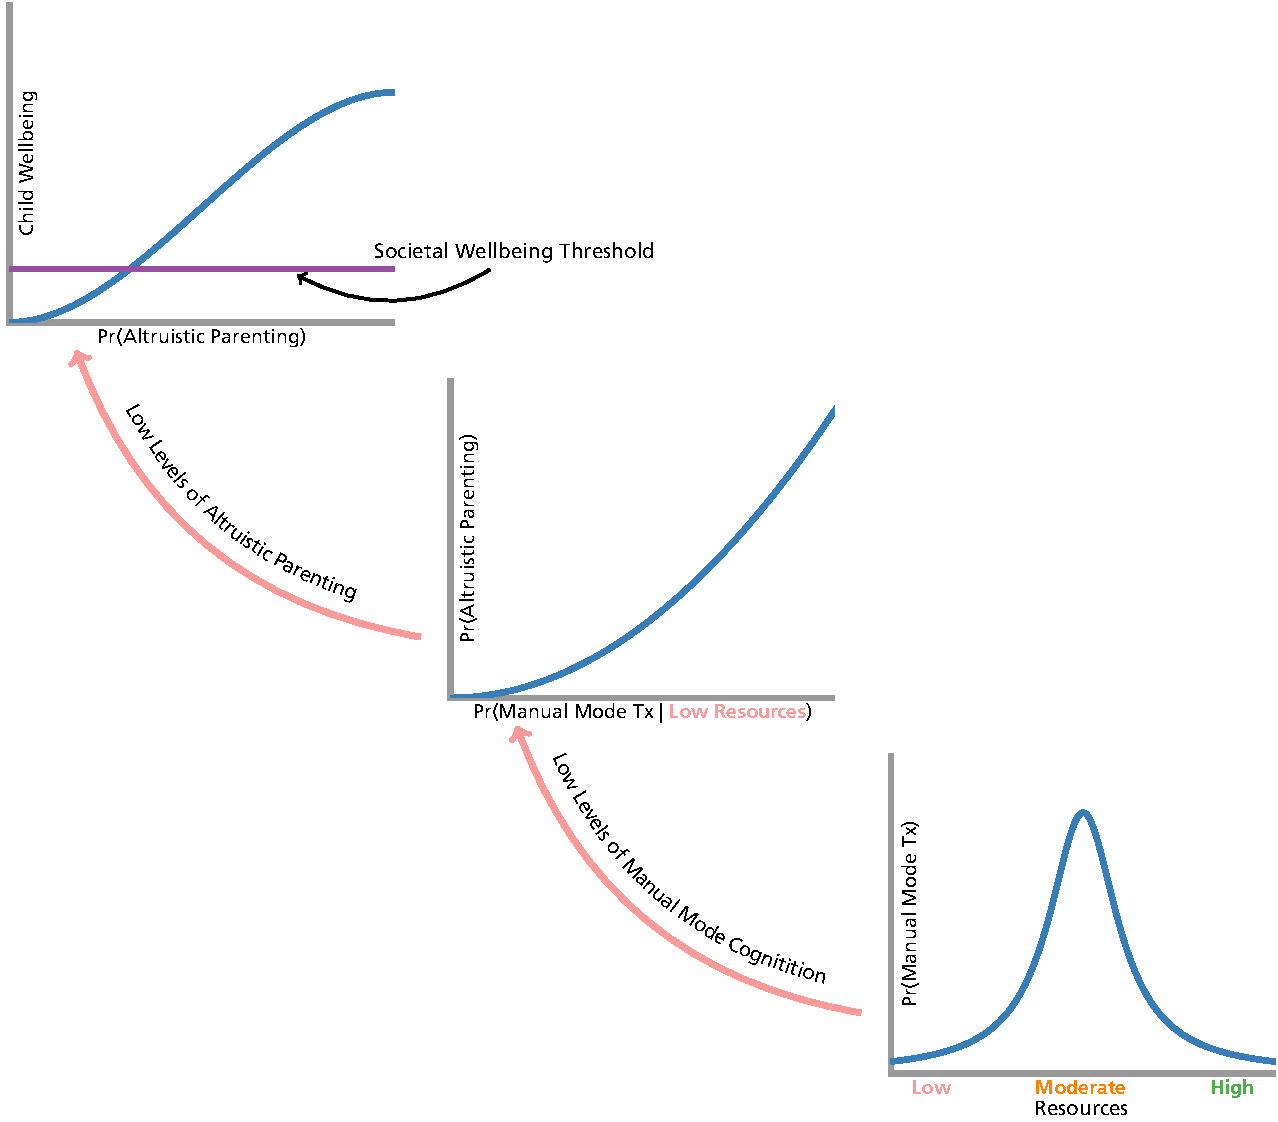
\includegraphics[scale=0.375]{general_conceptual_model_graphs.pdf}}

\end{frame}

\begin{frame}{Measuring Decision Making in Parents}

\begin{block}{Altruism}

Those parental behaviors or decisions requiring the investment of time
or other resources in a child in a way that increases the wellbeing of
the child but at a cost to parental wellbeing.

\end{block}

\begin{block}{Maltreative Behaviors}

Those behaviors that will ultimately bring a child's cumulative
well-being below the societally defined threshold.

\end{block}

\end{frame}

\begin{frame}{Connecting Altruism to Maltreative Parental Behaviors}

\centering{
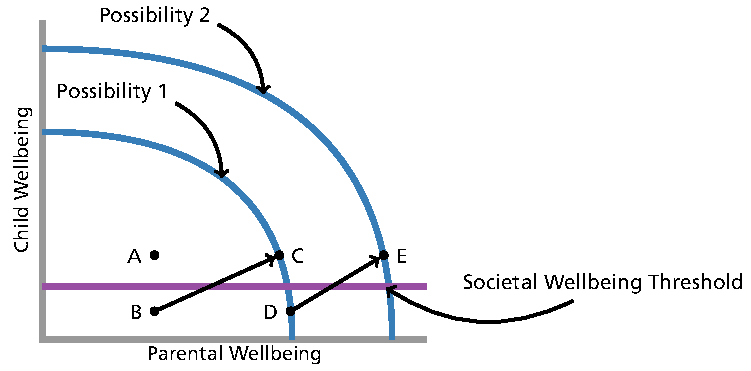
\includegraphics[scale=.9]{wellbeing_production_possibilities.pdf}}

\end{frame}

\begin{frame}{Major Predictions of the Model}

\begin{itemize}[<+->]
\itemsep1pt\parskip0pt\parsep0pt
\item
  As resource levels increase, maltreative parenting behavior will
  decrease (well-established).
\end{itemize}

\begin{itemize}[<+->]
\itemsep1pt\parskip0pt\parsep0pt
\item
  In the current analysis, an independent effect of altruism while
  controlling for the effects of resources is expected.
\end{itemize}

\end{frame}

\begin{frame}{Analytic Approach}

\begin{itemize}[<+->]
\itemsep1pt\parskip0pt\parsep0pt
\item
  Using data from the National Survey of Early Childhood Health (NSECH),
  the Consumer Expenditure Survey (CES), and the American Time Use
  Survey (ATUS), estimates of altruism, parental efficiency, income, and
  other control variables were calculated.
\end{itemize}

\begin{itemize}[<+->]
\itemsep1pt\parskip0pt\parsep0pt
\item
  A dependent measure of the probability that all reported discipline
  strategies would be Type-II strategies was also calculated.
\end{itemize}

\begin{itemize}[<+->]
\itemsep1pt\parskip0pt\parsep0pt
\item
  All variables were subjected to Bayesian Model Averaging (BMA) across
  quasibinomial GLMs to determine the most probable set of covariates.
  The BMA results estimate that the model with the highest posterior
  probability is a model which only includes the household and parental
  investments (household altruism) and the natural logarithm of their
  annual income.
\end{itemize}

\end{frame}

\begin{frame}{Model Results}

\centering{
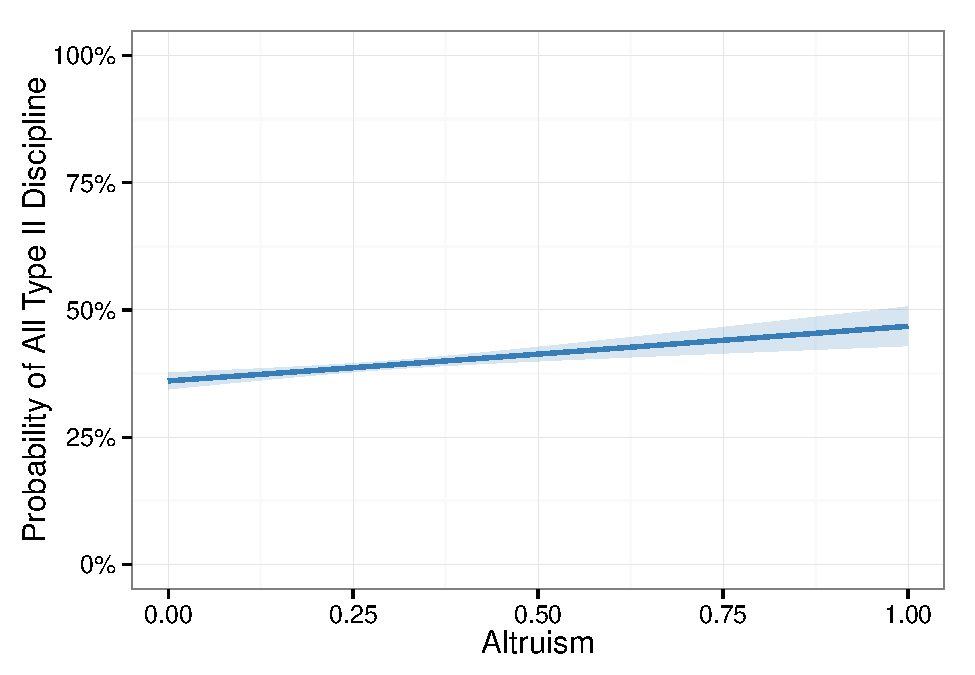
\includegraphics[scale=.65]{./qualpaper_v5_files/figure-latex/ModelResultGph2.pdf}}

\end{frame}

\begin{frame}{Discussion}

\begin{itemize}[<+->]
\itemsep1pt\parskip0pt\parsep0pt
\item
  The results of the analysis presented above confirm the hypothesis
  that more altruistic households will tend to engage in parenting
  strategies associated with wellbeing to a greater extent than less
  altruistic households.
\end{itemize}

\begin{itemize}[<+->]
\itemsep1pt\parskip0pt\parsep0pt
\item
  To the extent that the other assumptions of the theoretical model
  hold, the results of this analysis suggest that relatively simple
  models of human behavior might be able to explain how families become
  involved with the child welfare system.
\end{itemize}

\end{frame}

\begin{frame}{Next Steps}

\begin{itemize}[<+->]
\itemsep1pt\parskip0pt\parsep0pt
\item
  Examination of state-level estimates of altruism.
\end{itemize}

\begin{itemize}[<+->]
\itemsep1pt\parskip0pt\parsep0pt
\item
  Directly test opther aspects of the model through the monetization of
  various parenting staretgies.
\end{itemize}

\begin{itemize}[<+->]
\itemsep1pt\parskip0pt\parsep0pt
\item
  Brain-imaging studies explicitly testing assumptions used from
  dual-process theory of morality.
\end{itemize}

\begin{itemize}[<+->]
\itemsep1pt\parskip0pt\parsep0pt
\item
  MIMIC approach to measuring altruism and maltreative behaviors.
\end{itemize}

\end{frame}

\begin{frame}{}

Thank You!

\end{frame}

\end{document}
